\subsection{Design optimization}

This structure can be, as opposed to the previous version, improved in terms of performance. The critical path of this scheme consists of 4 combinatorial blocks, two multipliers and two adders, though by means of the appropriate transformations it is possible to reduce the longest combinatorial path.  In \autoref{fig:IIR_advanced_2} it has been identified the first cut-set that allows to move the register by changing the length of the critical path from 4 to 3.

\begin{figure}[htb]
	\center
	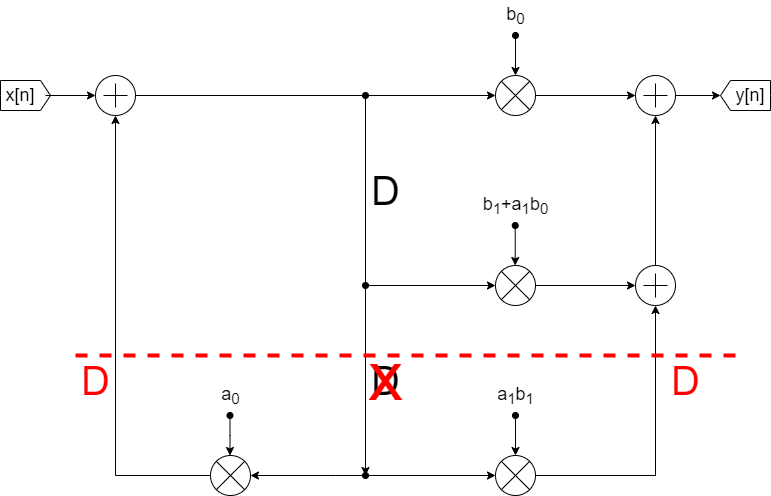
\includegraphics[width=0.55\textwidth]{IIR_2_1.png}
	\caption{Advanced architecture with $1^{st}$ transformation}
	\label{fig:IIR_advanced_2}
\end{figure}

In \autoref{fig:IIR_advanced_3} a feed-forward cut-set has been identified where it is possible to insert a pipeline stage on all three branches. In this way the combinatorial path including the $b_0$ multiplier is no longer part of the critical path. The longest combinatorial path includes the multiplier for the term $b_1 + a_1b_0$, the intermediate adder and the final adder. A further transformation allows to move the register from one side of the multiplier to the other without altering the behavior of the circuit, as in \autoref{fig:IIR_advanced_4}.

\begin{figure}[ht]
	\begin{minipage}[b]{0.5\linewidth}
		\centering
		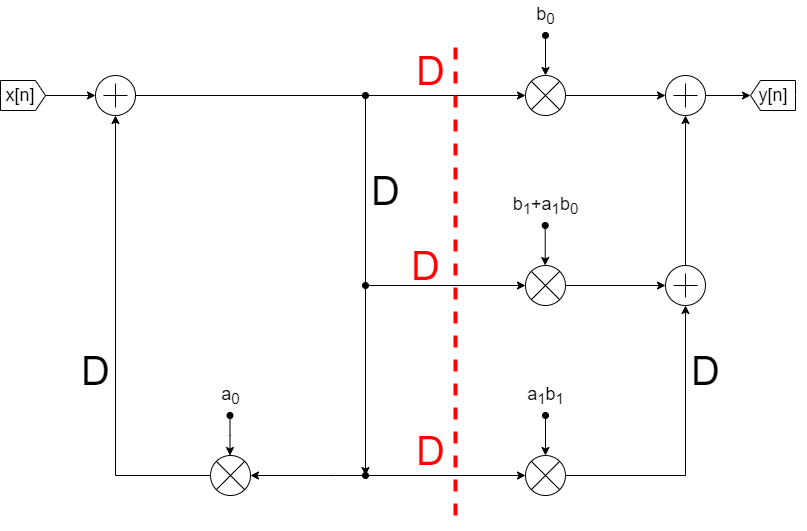
\includegraphics[width=\textwidth]{IIR_2_2.png}
		\caption{Advanced architecture with $2^{nd}$ transformation}
		\label{fig:IIR_advanced_3}
	\end{minipage}
	\hspace{0.5cm}
	\begin{minipage}[b]{0.5\linewidth}
		\centering
		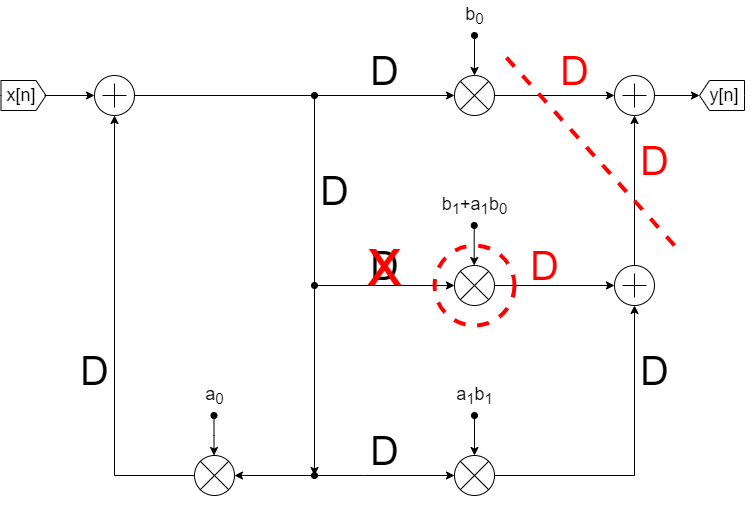
\includegraphics[width=\textwidth]{IIR_2_3.png}
		\caption{Advanced architecture with $3^{rd}$ transformation}
		\label{fig:IIR_advanced_4}
	\end{minipage}
\end{figure}

The latter transformation in \autoref{fig:IIR_advanced_4} takes into account the feed-forward cut-set on the two input branches at the last adder and through the insertion of a pipeline stage bring the critical path to be equal to the delay of a single multiplier.

In \autoref{fig:IIR_final} the optimized architecture of the IIR filter can be observed, in which a pipeline stage has been inserted between each combinatorial block. These transformations allow the circuit to reach the maximum throughput at the expense of latency, which compared to the initial circuit has increased from $2\,T_{ck}$ to $4\,T_{ck}$.

\begin{figure}[htb]
	\center
	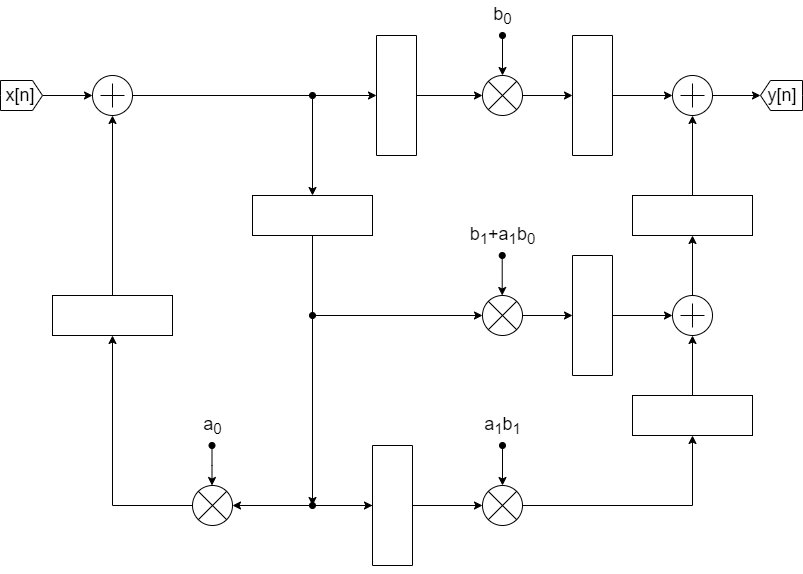
\includegraphics[width=0.65\textwidth]{IIR_final.png}
	\caption{Optimized architecture of J-look-ahead IIR filter}
	\label{fig:IIR_final}
	\end{figure}

\pagebreak